\chapter{Návrh grafického programovacieho jazyka}
\label{kap:navrh-gpj}

Kapitola pojednáva o voľbe vhodných technológii pre implementáciu jednotlivých cieľov práce. Detailom implementácie s použitím tu opísaných technológií je venovaná nasledujúca kapitola \ref{kap:implementacia}.

%%%%%
% %%% Editor kódu
%%%%%
\section{BlaBlaBla}
%Funkčnosť knižnice je založená na definícii blokov a im prislúchajúcich generátorov. Bloky sú navonok vizuálnym komponentom editora, ich spájaním tvorí používateľ kód. Súčasťou ich definície sú validátory, vykonávajúce kontroly (najmä typové). Validátory určujú obmedzenia použitia blokov, ľubovoľné dva bloky nemusí byť možné spojiť, čím možno vynútiť syntaktické pravidlá cieľového textového programovacieho jazyka. Každému bloku je tiež priradený generátor, ktorý zodpovedá za interpretáciu bloku pri generovaní výsledného kódu (u nás napríklad v jazyku C). Knižnica Blockly poskytuje základné, všeobecné bloky. K dispozícii sú bloky pre \textit{podmienku if}, \textit{cykly}, bloky pre \textit{logické a číselné konštanty} a manipuláciu s nimi (porovnávanie, sčítavanie, negácia a iné), bloky pre \textit{manipuláciu s textom}, \textit{tovrbu zoznamov}, \textit{reprezentáciu a miešanie farieb}, \textit{tvorbu premenných} a \textit{definíciu procedúr a funkcií}. Súčasťou sú generátory pre jazyky JavaScript, Python, Dart, Lua a PHP.

V knižnici dotvárame bloky reprezentujúce funkcie robota umožňujúce pohyb, čítanie hodnôt meraných senzormi, sériovú komunikáciu či komunikáciu rozhraním bluetooth. Komplexitou funkcie poskytovanej blokom je možné nastaviť úroveň abstrakcie. Jednoduchým príkladom je blok \uv{čakanie na stlačenie tlačidla} (obrázok \ref{obr:wait-till-couch}). Možno ho ľahko vyskladať z blokov \textit{cyklu while}, \textit{negácie} a bloku pre \textit{načítanie stavu tlačidla}, no najmä pre nižšie vekové kategórie je vhodnejšia alternatíva vyššej abstraktnej úrovene. Iným príkladom je blok pre načítanie gesta pomocou ultrazvukového senzora, ktorý reprezentuje v pozadí pomerne zložitú implementáciu časti riadiaceho programu, zabezpečujúcu komunikáciu s hardvérom a elimináciu chyby opakovaným meraním.

\begin{figure}
\centerline{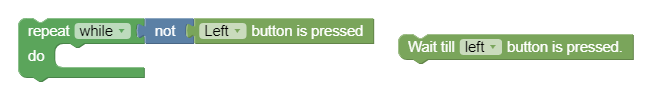
\includegraphics[width=1\textwidth]{images/wait-till-couch}}
\caption[Blockly --- abstrakcia bloku \uv{čakaj na stlačenie tlačidla}]{Blockly --- abstrakcia bloku \uv{čakaj na stlačenie tlačidla}}
\label{obr:wait-till-couch}
\end{figure}

Syntax jazyka C vyžaduje redefiníciu generátorov viacerých prebraných blokov. Vytvárame tiež generátory pre novo konštruované bloky. Usporiadaním v editore kódu sú použité bloky organizované v grafovej štruktúre, generátor je funkcia, ktorej parametrom je blok, na ktorom je volaná. Má prístup k poliam bloku (polia sú prvky pre výber možností, prípadne textový alebo číselný vstup, napríklad blok vpravo na obrázku \ref{obr:wait-till-couch} má pole na výber jednej z dvoch možností, \uv{left} a \uv{right}). Zároveň má generátor prístup k vnoreným blokom (napríklad blok cyklu while má prístup k blokom v tele cyklu) a pripojeným \uv{nasledovníkom} --- bloku pod ním. Návratovou hodnotou je vhodne spracovaný kód so zakomponovaným obsahom potomkov a polí. Kód je generovaný rekurzívne, zvyčajne začínajúc na najvyššom bloku umiestnenom v editore. V našej aplikácii je súčasťou editora fixný blok \uv{program}, ktorý reprezentuje časť \textit{loop} programu v Arduino a kód je tvorený pridávaním blokov do jeho tela. Bloky bez pripojenia (aj nepriameho) k tomuto bloku nie sú pri vyhodnocovaní brané do úvahy. Výnimku majú len bloky umiestnené v tele blokov definujúcich funkcie a procedúry. Príklad možno vidieť na obrázku \ref{obr:disabled-orphan-block}.

\begin{figure}
\centerline{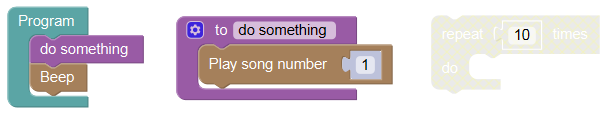
\includegraphics[width=0.65\textwidth]{images/disabled-orphan-block}}
\caption[Blockly --- blok pre riadiaci program robota]{Blockly --- blok pre riadiaci program robota}
\label{obr:disabled-orphan-block}
\end{figure}

Dôležitým komponentom jazyka sú premenné. Blockly je potrebné prispôsobiť pre použitie typových premenných jazyka C, pričom autori podobných aplikácií pristupujú k riešeniu rôzne. V online webovej verzií editora MakeCode (riadenie robota Lego Mindstorms) sú k dispozícii len číselné premenné, textové reťazce a binárne hodnoty môžu byť len konštantou \cite{makeCodeWebEditor}. Na druhej strane, v produkte Otto Blockly je možné vytvoriť premennú typu znak, reťazec, celé číslo, desatinné číslo i binárna hodnota. K dispozícií sú bloky pre inicializáciu, priradenie, i získanie hodnoty premennej. Typy nie sú však vizuálne výraznejšie odlíšené. V editore kódu možno deklarovať premennú binárneho typu a následne iným blokom túto premennú inkrementovať, na čo validátor bloku oznámi chybu. Otázne však je, či je vhodné povoliť vytvorenie neprípustného spojenia. V našej aplikácii vynucujeme určenie typu premennej pri jej vytváraní, bez možnosti dodatočnej zmeny. Povolené typy sú celé číslo (int16\_t), textový reťazec (String) a binárna hodnota (bool). Bloky pre priradenie do premennej a čítanie premennej majú v rámci typu rovnakú farbu.